\section{Introduction}

Ecological resources are often managed on the basis of outputs derived
from models of species-environment relationships, variously referred to
as: habitat suitability models, species distribution models, resource
selection functions, or ecological niche models. Therefore, evaluating
the predictive ability of such models is a necessary prerequisite for
robust decision-making. While such evaluations are ideally based on
independent data collected purely for the purpose of model testing, in
ecological studies fully independent data is often unavailable due to
logistical or financial constraints. Therefore, statistical resampling
methods are the most important tool we have for evaluating predictive
ability.

\bigskip

To briefly summarise, resampling methods repeatedly resample the full
dataset to create training and testing data subsets that are independent
of one another. The model is then iteratively fit using each training
data subset and prediction error estimated using the independent testing
data subset. An overall estimate of prediction error is then calculated
as the average prediction error across all resampled data subsets. While
resampling methods are not a replacement for independent data, they can
be used to conduct an internal evaluation that penalises for optimism
from overfitting\supercite{verbyla-1989}.

\bigskip

In their seminal paper on model evaluation Fielding and Bell\supercite{fielding-1997}
state with reference to resampling methods ``The
ecological literature seems to have paid little attention to how the
partitioning method can influence the error rates. Verbyla and Litvaitis
briefly reviewed a range of partitioning methods in their
assessment of resampling methods for evaluating classification
accuracy.'' The work of Verbyla and Litvaitis\supercite{verbyla-1989} remains the
only comparison of resampling methods for evaluating species-environment
relationship models. Therefore, given the importance of this work, we
endeavoured to replicate the study using an open computational approach.

\section{Prediction error}

When developing a species-environment relationship model, we will
usually have a dataset $d$ that contains observations or measurements
that form a species response variable $y$ and a set of one or more
environmental explanatory variables $x$. Using a species-environment
relationship model function $f^{}$ trained on the dataset $f^{(d)}$ a
prediction of the response variable $\hat{y}$ can be created from the
environmental explanatory variables for each sample $i$:

\begin{equation}
\hat{y_i} = f^{(d)}(x_i)
\end{equation}

We can then define the prediction error $Err$ for each sample $i$ as the
absolute difference between the observed response variable $y_i$ and
predicted response variable $\hat{y_i}$:

\begin{equation}
Err_i = | y_i - \hat{y_i} |
\end{equation}

This definition of $Err$ is equivalent to the binary misclassification
error rate used by Verbyla and Litvaitis\supercite{verbyla-1989}, as when
$y_i = \hat{y}$ then $Err_i = 0$, and when $y_i \neq \hat{y}$ then
$Err_i = 1$. But by expressing $Err$ in these terms generalises the
approach to situations in which the species-environment relationships
are measured or modelled on a continuous rather than binary scale, which
has become more common practice since the original computational
experiment was conducted.

\section{Resampling methods}

During the replication process it became apparent that the terminology
for resampling methods has developed over time, and has been used
somewhat inconsistently. Therefore, we begin by naming and formally
defining each of the resampling methods we have used based on
descriptions within the references.

\subsection{Resubstitution}

Given a dataset $d$ of size $n$ the resubstitution method calculates the
mean prediction error across all samples $i$ from a modelling function
trained on the entire dataset $f^{(d)}$.

\begin{equation}
Err^{R} = \frac{1}{n} \sum_{i=1}^{n} | y_i - f^{(d)}(x_i) |
\label{eq:resubstitution}
\end{equation}

The value $Err^{R}$ is called the resubstitution (or apparent) error
rate and is likely to provide an optimistic estimate of prediction
error, as the same data is used to train and test the model.

\subsection{Hold-out cross-validation}

Hold-out (or: split-sample, randomised, Monte Carlo) cross-validation
randomly partitions the dataset into training and testing subsets. 
Verbyla and Litvaitis\supercite{verbyla-1989} referred to this approach as 
simply ``cross-validation'' but we have chosen to use the more specific 
term of hold-out cross-validation to clarify which of the many types of 
cross-validation we are referring to. The proportion $p$ of data `held-out' 
from the dataset $d$ forms a testing
dataset $t$ of sample size $\sharp t$, with the remaining data forming
training dataset $\{d-t\}$. The model is fitted using the training
dataset $f^{(\{d-t\})}$, and the prediction error is estimated as the
mean prediction error for all $i$ in $t$ across a number of $H$
repetitions.

\begin{equation}
Err^{H}_{p} = \frac{1}{H } \sum_{t=1}^{H} \frac{1}{\sharp t} \sum_{i \in t} | y_i - f^{(\{d-t\})}(x_i) |
\end{equation}

In general this method can be considered an improvement over
resubstitution as the data used to train the model is separated from the
data used to test the model.

\subsection{$K$-fold cross-validation}

Verbyla and Litvaitis\supercite{verbyla-1989} describe a resampling method called ten-fold
cross-validation and another method called $n$-fold cross-validation or the jackknife.
Both these methods are variations of $K$-fold cross-validation. The $K$-fold
cross-validation method begins by randomly partitioning the
dataset into $k$ equally sized sets. Then the prediction for each sample
$i$ is calculated from a model fitted to the set $\{d-k : i \in k\}$,
which is the dataset $d$ excluding the set $k$ where $k$ includes $i$.

\begin{equation}
Err^{K}  = \frac{1}{n} \sum_{i=1}^{n} | y_i - f^{(\{d-k : i \in k\})}(x_i) |
\end{equation}

When $k = n$ then we produce a special form of $K$-fold cross-validation
called the jackknife (or: leave-one-out, $n$-fold) cross-validation.

\subsection{Bootstrap cross-validation}

Bootstrapping\supercite{diaconis-1983} is based upon a set $B$ of bootstrap sample datasets $b$,
for which $b$ is of size $n$ and is generated by randomly sampling with
replacement from the full dataset $d$. The model is
iteratively fitted to each $b$ and prediction errors calculated for all
samples $i$ in the test set $\{d - b\}$ that consists of the dataset $d$ with
all the $i$ in the bootstrap sample $b$ removed. This results in around
0.632 of the dataset $d$ occurring at least once in the training set $b$,
and the remaining 0.368 of $d$ occurring in testing set\supercite{hastie-2009}. The estimated prediction error rate is then the mean
prediction error across all bootstrap samples\supercite{efron-1983, jain-1987}.

\begin{equation}
Err^{B} = \dfrac{\sum\limits_{b=1}^{B}\sum\limits_{{i \in \{ d-b \} }}| y_i - f^{(b)}(x_i) |}{\sum\limits_{b=1}^{B} \sharp \{ d-b \}}
\label{eq:original-bootstrap}
\end{equation}

It is worth noting in the context of a replication study that the
equation used to calculate $Err^{B}$ was later changed, as this caused
some confusion during our replication. The second equation\supercite{efron-1993} works through
each sample $i$, and calculates the mean prediction error for a set
$C_i$ of size $\sharp C_i$ that is equal to the all bootstrap samples
that do not contain $i$, $C_i = \{ b \in B : i \notin b \}$.

\begin{equation}
Err^{B} = \frac{1}{n} \sum_{i=1}^{n} \frac{1}{\sharp C_i} \sum_{b \in C_i} | y_i - f^{(b)}(x_i) |
\end{equation}

This second definition was later termed the `leave-one-out bootstrap'
where it was also noted by Efron\supercite{efron-1997} that these ``two definitions agree as
$B \rightarrow \infty$ and produced nearly the same results in our
simulations'' which were based on $B=50$. Although the later
defintion of $Err^{B}$ has become more commonly used\supercite{hastie-2009}, 
as the two methods produce nearly identical results, we
have used the original definition (Equation \ref{eq:original-bootstrap})
in our replication as it is simpler to compute, and was the version used
by Verbyla and Litvaitis\supercite{verbyla-1989} that we are trying to replicate.

\section{Computational experiment replication}

Verbyla and Litvaitis\supercite{verbyla-1989} based their computational experiment
on applying linear discriminant analysis models to a random dataset.
Their premise was that by creating a random dataset the predictive
ability of a model should be no better than chance, and hence as the
true prediction error was known exactly each resampling method could be
assessed for bias and precision.

\subsection{Random datasets}

Each of 1000 computational experiments began by creating a random
dataset. The response variable consisted of 30 observations that were
randomly assigned a presence $=1$ or absence $=0$ value. These 30
observations were then matched with 10 explanatory variables. Verbyla and Litvaitis\supercite{verbyla-1989} 
state that the ``ten predictor variables were
generated with univariate normal distributions and equal variances'' but
neither the mean nor variance used was reported. Therefore, we assumed a
standard normal distribution of $\mu$ = 0 and $\sigma$ = 1. For each random
dataset a linear discriminant analysis model was fitted and prediction error
calculated using each resampling method.

\subsection{Resubstitution}

The resubstitution method is the simplest approach and the most
consistently reported in the literature, therefore we applied the
methodology exactly as described.

\subsection{$K$-fold cross-validation)}

We conducted $K$-fold cross-validation with $K=10$ and $K=n$ as in
Verbyla and Litvaitis\supercite{verbyla-1989} -- remembering that $K=n$ is
equivalent to the jackknife method. We also included $K=3$ as this
represents a situation with a similar proportion of the dataset forming
training and testing sets as with the bootstrap. This was done to assess
if the proportion of data within training and testing sets was affecting
comparisons of the resampling methods.

\subsection{Bootstrap cross-validation}

The bootstrap method was applied with bootstrap samples $B=200$ as
specified in the example code provided by Verbyla and Litvaitis\supercite{verbyla-1989}.

\subsection{Hold-out cross-validation}

We included three cases of hold-out cross-validation as while Verbyla and Litvaitis\supercite{verbyla-1989} 
stated that for this method the ``the estimate
of model classification accuracy will not be very precise'' no
experiments or citations were provided to support this claim. In
addition we felt there was some inconsistency in the two citations given with
reference to this method.  While Verbyla and Litvaitis\supercite{verbyla-1989} state 
``only one estimate of accuracy 
is made'' which matches the citation\supercite{lachenbruch-1968} using hold-out cross-validation
with $H=1$, a second citation\supercite{capen-1986} referred to hold-out
cross-validation with $H=10$.  Given this uncertainty we
explored three different versions of hold-out cross-validation. We used
$p=0.368$ twice to match the proportion of test data in the bootstrap
approach, and with $H=1$ for one method, and $H=200$ in the second
method for consistency with the bootstrap. We also used $H=200$ with
$p=0.200$ to examine sensitivity to the test data proportion.

\section{Results}

The results for each resampling method were presented by Verbyla and Litvaitis\supercite{verbyla-1989} 
as a ``smoothed frequency distribution'' but the
smoothing method was not reported. As their results appeared to be
normally distributed, to mimic the original results to aid comparisons
we produced our smoothed distributions using a one-dimensional Gaussian
kernel density estimator with a bandwidth of one (Figure \ref{fig:smoothed-distributions}).

\begin{figure}[tbh]
\centering
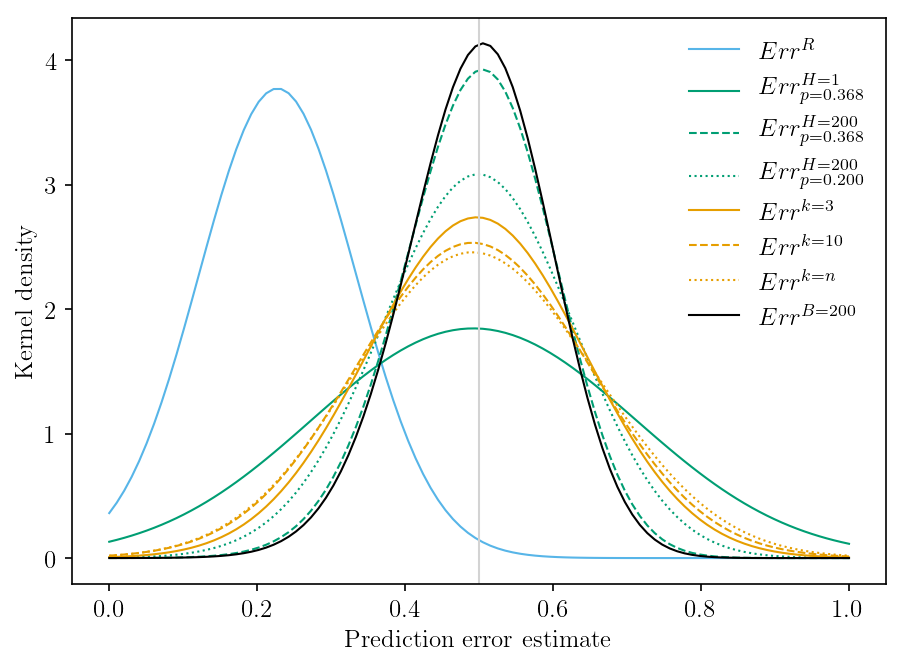
\includegraphics[width=\textwidth]{../code/resampling-results.png}
\caption{Smoothed distributions of estimates of prediction error for various resampling methods from 1000 computational experiments with the known prediction error of 0.5 also marked.}
\label{fig:smoothed-distributions}
\end{figure}

\bigskip

Looking at the distribution of $Err$ across the 1000 computational
experiments, the resubstitution method produced clearly biased estimates
of prediction error. All the other methods produced unbiased estimates,
but there was notable variation in the precision of those estimates,
with $Err^{B=200}$ ($\mu=0.497$, $\sigma=0.069$) producing the most
precise estimates.

\section{Conclusion}

While a lack of method description means our implementation will be
different to that of Verbyla and Litvaitis\supercite{verbyla-1989}, we would
conclude that our results are sufficiently similar to have replicated
their computational experiments.

\bigskip

Our findings confirm that resubstitution is a biased estimate of
prediction error, and that bootstrap cross-validation produces the most
precise unbiased estimate. We also found that hold-out cross-validation
produced unbiased but highly variable estimates of $Err$ as the method
is clearly sensitive to the choice of parameters. We found little
difference between any of the $K$-fold cross-validation methods.

\bigskip

Given the findings from our replication, we would support Verbyla and Litvaitis\supercite{verbyla-1989} 
in advocating the use of the bootstrap, as it
produced the most precise estimate, and unlike other resampling methods
it does not require a arbitrary choice of dataset partitions or splits
that could confound inter-study comparisons of model evaluations.

\bigskip

We conclude that while not a substitute for truly independent data,
resampling methods should be considered an important part of
species-environment relationship model evaluation, and would encourage
the use of the bootstrap cross-validation method in particular.

\section{Acknowledgements}

This research was funded by internal investment by Manaaki Whenua –
Landcare Research.





















